\chapter{Embedded Computer Setup}
\label{ap: appendixD}

This appendix describes the steps required to connect an embedded computer to the iBEMS Core. 

\section{Connect to router}
In our project, we used a BeagleBone Blue for the embedded computer. To connect to your specific router, first plug in the BeagleBone Blue to your computer with a microUSB cable. Then open a terminal and install \say{screen} with the command \say{sudo apt install screen}. You will then need to find the USB driver being used for the beaglebone with \say{dmesg}. Scroll through the information until you find the BeagleBone:

\begin{figure}[H]
\centering
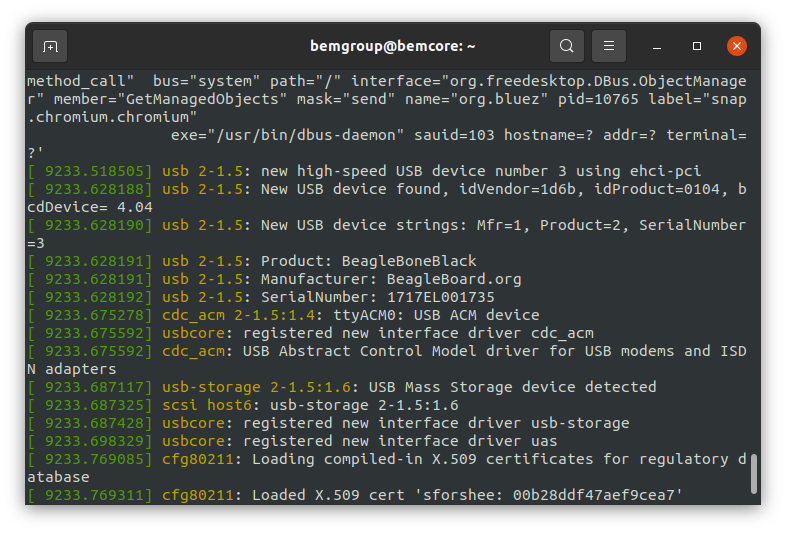
\includegraphics[scale=0.4]{figs/beaglebone/findUSBdriver.png}
\caption{Finding USB Driver}
\label{fig:bb_findUSB}
\end{figure}

In Figure~\ref{fig:bb_findUSB}, it can be seen that \say{ttyACM0} is the USB driver being used.

With that knowledge, you can now enter the command \say{sudo screen /dev/ttyACM0} to login into the Beaglebone Blue. Enter username \say{debian} and password \say{temppwd} to login.
\medbreak
Once you are logged into the Beaglebone Blue, follow these instructions to connect to your router:
\href{http://www.strawsondesign.com/\#!manual-wifi}{http://www.strawsondesign.com/\#!manual-wifi}.

\section{Copy Necessary Files}
Now that the Beaglebone Blue is connected to the router, you need to copy some files to it. First, find the IP address of the BeagleBone Blue with the command \say{ifconfig wlan0}:

\begin{figure}[H]
\centering
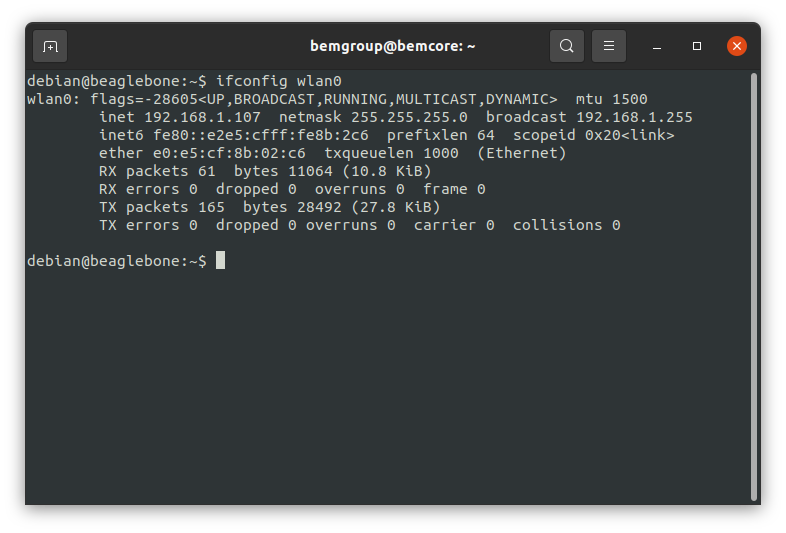
\includegraphics[scale=0.4]{figs/beaglebone/findIPaddress.png}
\caption{Finding IP Address}
\label{fig:bb_findIP}
\end{figure}

Figure~\ref{fig:bb_findIP} shows the output of \say{ifconfig wlan0} and it can be seen that the IP address in this case is \texttt{192.168.1.107}.
\medbreak
You can now open a new native linux terminal and go the the \say{seniorProject1-2020-21-Code} directory. Once there, copy the necessary files with commands:
\\
\say{scp BeagleboneReceiver.py debian@192.168.1.107:/home/debian},
\\
\say{scp BeagleBoneSupportFiles/LED.py debian@192.168.1.107:/home/debian},
\\
\say{scp BeagleBoneSupportFiles/PWM.py debian@192.168.1.107:/home/debian}.
You may get a warning message about the authenticity of the host, but simply type \say{yes} as response to this warning.

\section{Running the BeagleBone Receiver}
With the necessary files on the BeagleBone Blue, you can go back the BeagleBone Blue terminal and enter the command \say{python3 BeagleboneReceiver.py}. Finally, you can start iBEMS and it will connect to the Beaglebone Blue automatically.